\documentclass[12pt,letterpaper]{article}
\usepackage[utf8]{inputenc}
\usepackage[spanish]{babel}
\usepackage{graphicx}
\usepackage[left=2cm,right=2cm,top=2cm,bottom=2cm]{geometry}
\usepackage{graphicx} % figuras
% \usepackage{subfigure} % subfiguras
\usepackage{float} % para usar [H]
\usepackage{amsmath}
%\usepackage{txfonts}
\usepackage{stackrel} 
\usepackage{multirow}
\usepackage{enumerate} % enumerados
\renewcommand{\labelitemi}{$-$}
\renewcommand{\labelitemii}{$\cdot$}
% \author{}
% \title{Caratula}
\begin{document}

% Fancy Header and Footer
% \usepackage{fancyhdr}
% \pagestyle{fancy}
% \cfoot{}
% \rfoot{\thepage}
%

% \usepackage[hidelinks]{hyperref} % CREA HYPERVINCULOS EN INDICE

% \author{}
\title{Caratula}

\begin{titlepage}
\begin{center}
\large{UNIVERSIDAD PRIVADA DE TACNA}\\
\vspace*{-0.025in}
\begin{figure}[htb]
\begin{center}

\includegraphics[width=7cm]{./images/logo}
\end{center}
\end{figure}
\vspace*{0.15in}
INGENIERIA DE SISTEMAS  \\

\vspace*{0.3in}
\begin{large}
\textbf{TITULO:} \\
\end{large}

\vspace*{0.1in}
\begin{Large}
\textbf{Informe de Laboratorio 01:Elaboración de Pruebas UnitariasArchivo} \\

\end{Large}

\vspace*{0.3in}
\begin{Large}
\textbf{CURSO:} \\
\end{Large}

\vspace*{0.1in}
\begin{large}
Calidad y Pruebas de Software\\
\end{large}

\vspace*{0.3in}
\begin{Large}
\textbf{DOCENTE:} \\
\end{Large}

\vspace*{0.1in}
\begin{large}
 Ing. Patrick Cuadros Quiroga\\
\end{large}

\vspace*{0.4in}
\vspace*{0.1in}
\begin{large}
\textbf{INTEGRANTES:} \\
\begin{flushleft}
Yaneth Virginia Aquino Huallpa \hfill	(2017059286)\\

\centering  %CENTRA UN TEXTO
\vspace*{0.9in}
\begin{large}
Tacna
\end{large}

\end{flushleft}
\end{large}
\end{center}

\end{titlepage}


\tableofcontents % INDICE
\thispagestyle{empty} % INDICE SIN NUMERO
\newpage
\setcounter{page}{1} % REINICIAR CONTADOR DE PAGINAS DESPUES DEL INDICE


\section{Crear un proyecto para pruebas} 
\begin{itemize}
 \item  Crear un proyecto nuevo de C char Aplicación de consola (.NET Core) y Asigne al proyecto el nombre Bank .
\item Crear un proyecto de prueba unitaria  de prueba de MSTest (.NET Core) de C char y  Ponga al proyecto el nombre BankTests.

\begin{center}
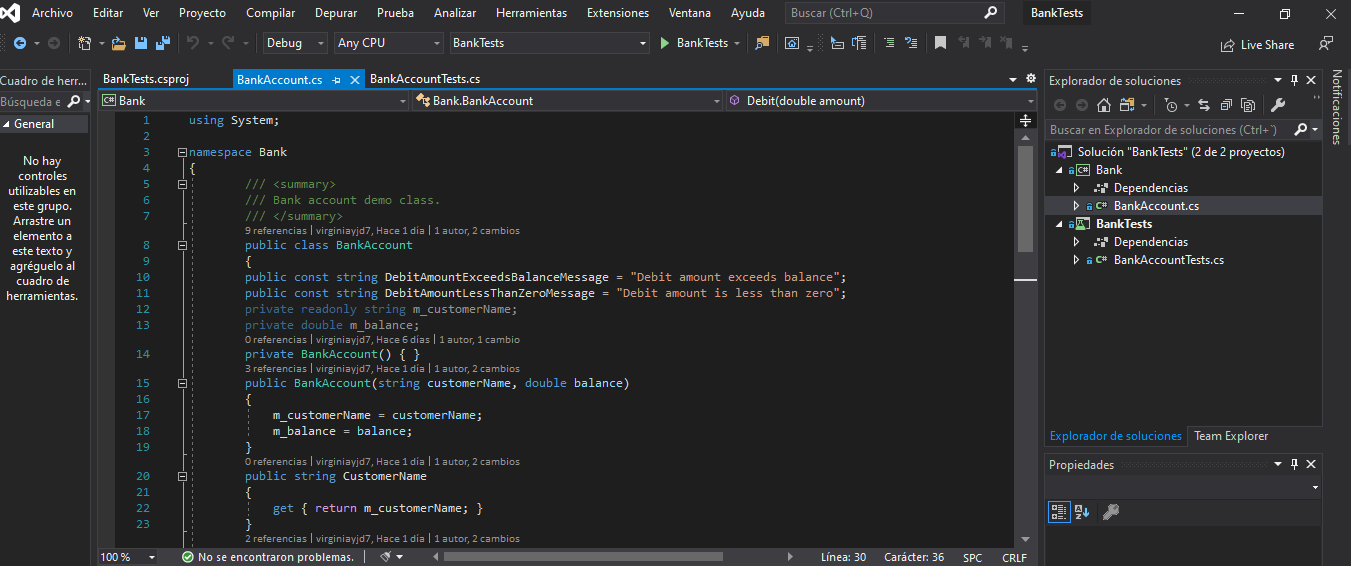
\includegraphics[width=\columnwidth]{images/1}\newline
\end{center}
\item Reemplace el contenido de Program.cs por el siguiente código de C char que define una
clase, BankAccount
\begin{center}
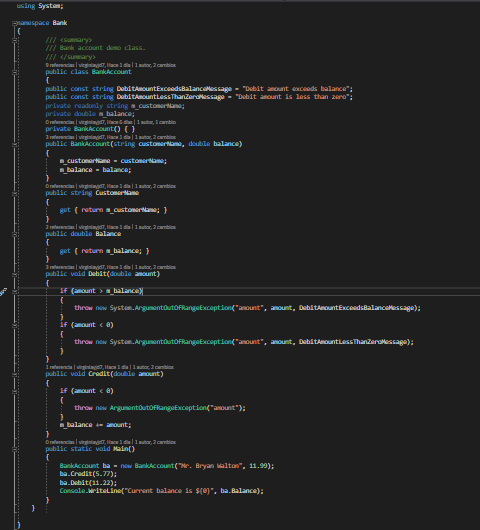
\includegraphics[width=\columnwidth]{images/2}\newline
\end{center}
\item El archivo BankAccountTests.cs contiene ahora el siguiente código:
\begin{center}
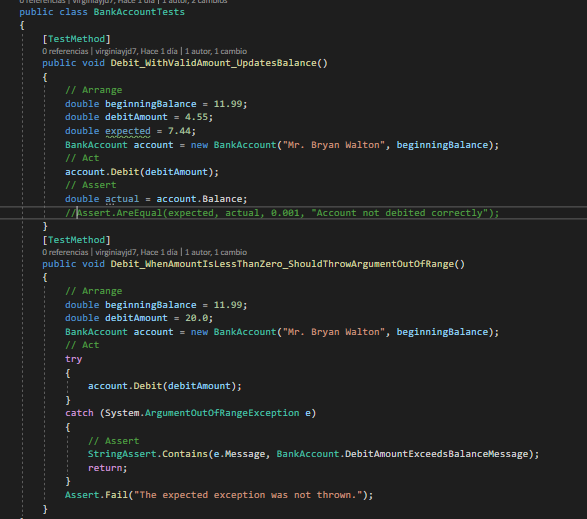
\includegraphics[width=\columnwidth]{images/3}\newline
\end{center}
\end{itemize}
\section{Resultado:Al  ejecutar la prueba, se muestra:} 
\begin{center}
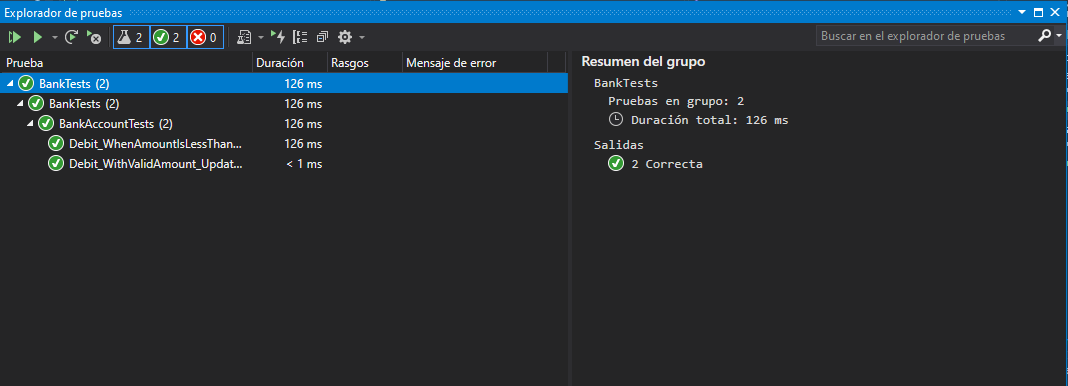
\includegraphics[width=\columnwidth]{images/final}\newline
\end{center}




\end{document}